\documentclass[12pt,A4paper,authoryear]{elsarticle} %review=doublespace preprint=single 5p=2 column
%%% Begin My package additions %%%%%%%%%%%%%%%%%%%
%% Other Customizations
\usepackage[hyphens]{url}
\usepackage{lineno} % add
\usepackage{caption}


\usepackage{setspace}
\setstretch{1.25}

\usepackage{mathpazo}


\providecommand{\tightlist}{%
  \setlength{\itemsep}{0pt}\setlength{\parskip}{0pt}}

\biboptions{sort&compress} % For natbib
\usepackage{booktabs} % book-quality tables

% Redefines the elsarticle footer
\makeatletter
\def\ps@pprintTitle{%
  \let\@oddhead\@empty
  \let\@evenhead\@empty
  \def\@oddfoot{\it \hfill\today}%
  \let\@evenfoot\@oddfoot}
\makeatother

% A modified page layout
\textwidth 6.75in
\oddsidemargin -0.15in
\evensidemargin -0.15in
\textheight 9in
\topmargin -0.5in
%%%%%%%%%%%%%%%% end my additions to header

\usepackage[T1]{fontenc}
\usepackage{amssymb,amsmath}

\usepackage{ifxetex,ifluatex}
\usepackage{fixltx2e} % provides \textsubscript
% use upquote if available, for straight quotes in verbatim environments
\IfFileExists{upquote.sty}{\usepackage{upquote}}{}
\ifnum 0\ifxetex 1\fi\ifluatex 1\fi=0 % if pdftex
\usepackage[utf8]{inputenc}

\usepackage[T1]{fontenc}
\usepackage{amssymb,amsmath}
\usepackage{ifxetex,ifluatex}
\usepackage{fixltx2e} % provides \textsubscript
% use upquote if available, for straight quotes in verbatim environments
\IfFileExists{upquote.sty}{\usepackage{upquote}}{}
\ifnum 0\ifxetex 1\fi\ifluatex 1\fi=0 % if pdftex
\usepackage[utf8]{inputenc}
\else % if luatex or xelatex
\usepackage{fontspec}
\ifxetex
\usepackage{xltxtra,xunicode}
\fi
\defaultfontfeatures{Mapping=tex-text,Scale=MatchLowercase}
\newcommand{\euro}{€}
\setmonofont{Source Code Pro}
\fi
% use microtype if available
\IfFileExists{microtype.sty}{\usepackage{microtype}}{}
\usepackage[margin=1in]{geometry}
\usepackage{natbib}
\bibliographystyle{plainnat}
\usepackage{longtable}
\ifxetex
\usepackage[setpagesize=false, % page size defined by xetex
unicode=false, % unicode breaks when used with xetex
xetex]{hyperref}
\else
\usepackage[unicode=true]{hyperref}
\fi

\setlength{\parindent}{0pt}
\setlength{\parskip}{6pt plus 2pt minus 1pt}
\setlength{\emergencystretch}{3em}  % prevent overfull lines
\setcounter{secnumdepth}{0}
% Pandoc toggle for numbering sections (defaults to be off)
\setcounter{secnumdepth}{0}
% Pandoc header


% \usepackage[nomarkers]{endfloat}

%% My customizations %%%%%%%%
%% Loading Packages
\usepackage[inline]{enumitem}
\usepackage{float}
\usepackage{tabularx}
\usepackage[dvipsnames]{xcolor}
\usepackage{pgf, tikz}
\usepackage{amsthm}

%% Custom macros
\newtheorem{mydef}{Definition}
\newcommand{\bs}[1]{\ensuremath{\boldsymbol{#1}}}
\newcommand{\diag}[1]{\mathrm{diag}\left(#1\right)}
\newcommand{\seq}[3][1]{\ensuremath{#2_{#1},\ldots,\,#2_{#3}}}
\newcommand{\note}[1]{\marginpar{\scriptsize\tt{\color{RoyalBlue}#1}}}
\newcommand{\edit}[1]{{\color{OrangeRed} #1}}

%% Custom Lengths
\setlength{\parindent}{0pt}
\setlength{\parskip}{9pt}

%% Define Colors
\newcommand\myshade{85}
\colorlet{mylinkcolor}{violet}
\colorlet{mycitecolor}{YellowOrange}
\colorlet{myurlcolor}{Aquamarine}

%% Hyperlink Setup
\AtBeginDocument{%
  \hypersetup{breaklinks=true,
    bookmarks=true,
    pdfauthor={},
    pdftitle={simrel-m: A versatile tool for simulating multi-response linear model data},
    colorlinks=true,
    urlcolor=myurlcolor!\myshade!black,
    linkcolor=mylinkcolor!\myshade!black,
    citecolor=mycitecolor!\myshade!black,
    pdfborder={0 0 0}}
}

\urlstyle{same}  % don't use monospace font for urls

%% End my customizations %%%%%%%%%

\begin{document}
\begin{frontmatter}

  \title{\texttt{simrel-m}: A versatile tool for simulating multi-response linear
model data}
    \author[]{Raju Rimal}
  
  
    \author[]{Trygve Almøy}
  
  
    \author[Norwegian University of Life Sciences]{Solve Sæbø\corref{c1}}
  
   \cortext[c1]{Dep. of Chemistry and Food Science, NMBU, Ås
(\href{http://nmbu.no}{nmbu.no})}
    
  \begin{abstract}
    \small
    Data science is generating enormous amounts of data, and new and
    advanced analytical methods are constantly being developed to cope with
    the challenge of extracting information from such ``big-data''.
    Researchers often use simulated data to assess and document the
    properties of these new methods, and in this paper we present
    \texttt{simrel-m}, which is a versatile and transparent tool for
    simulating linear model data with extensive range of adjustable
    properties. The method is based on the concept of relevant components
    \citet{helland1994comparison}, which is equivalent to the envelope model
    \citet{cook2013envelopes}. It is a multi-response extension of
    \texttt{simrel} \citet{saebo2015simrel}, and as \texttt{simrel} the new
    approach is essentially based on random rotations of latent relevant
    components to obtain a predictor matrix \(\mathbf{X}\), but in addition
    we introduce random rotations of latent components spanning a response
    space in order to obtain a multivariate response matrix \(\mathbf{Y}\).
    The properties of the linear relation between \(\mathbf{X}\) and
    \(\mathbf{Y}\) are defined by a small set of input parameters which
    allow versatile and adjustable simulations. Sub-space rotations also
    allow for generating data suitable for testing variable selection
    methods in multi-response settings. The method is implemented as an
    R-package which serves as an extension of the existing \texttt{simrel}
    packages \citet{saebo2015simrel}.
  \end{abstract}
   \begin{keyword} \footnotesize \texttt{simrel-2.0}, \texttt{simrel} package in r, data
simulation, linear model, \texttt{simrel-m} \sep \end{keyword}
\end{frontmatter}

\section{Introduction}\label{introduction}

Technological advancement has opened a door for complex and
sophisticated scientific experiments that was not possible before. Due
to this change, enormous amounts of raw data are generated which
contains massive information but difficult to excavate. Finding
information and performing scientific research on these raw data has now
become another problem. In order to tackle this situation new methods
are being developed. However, before implementing any method, it is
essential to test its performance. Often, researchers use simulated data
for the purpose which itself is a time-consuming process. The main focus
of this paper is to present a simulation method, along with an r-package
called \texttt{simrel-m}, that is versatile in nature and yet simple to
use.

The simulation method we are presenting here is based on the principal
of relevant space for prediction \citep{helland1994comparison} which
assumes that there exists a subspace in the complete space of response
variables that is spanned by a subset of eigenvectors of predictor
variables. The r-package based on this method lets user specify various
population properties such as which components of predictors
\((\mathbf{x})\) are relevant for a latent subspace of the responses
\(\mathbf{y}\) and collinearity structure of \(\mathbf{x}\). This
enables the possibility to construct data for evaluating estimation
methods and methods developed for variable selection.

Among several publications on simulation
({\color{red}\texttt{which\ publications}}),
\citet{ripley2009stochastic} has exhaustively discussed the topic. In
addition, many publications ({\color{red}\texttt{which\ publications}})
are available on studies which has implemented simulated data in order
to investigate new estimation methods and prediction strategy
\citep[see:][]{cook2015simultaneous, cook2013envelopes, helland2012near}.
However, most of the simulations in these studies were developed to
address their specific problem. A systematic tool for simulating linear
model data with single response, which could serve as a general tool for
all such comparisons, was presented in \citet{saebo2015simrel} and as
the r-package \texttt{simrel}. This paper extends \texttt{simrel} in
order to simulate linear model data with multivariate response with an
r-package \texttt{simrel-m}.

\section{Statistical Model}\label{statistical-model}

Let us consider a model in
equation\textasciitilde{}\eqref{eq:rand-reg-model} as our point of
departure.

\begin{equation}
  \begin{bmatrix}\mathbf{y}\\ \mathbf{x}\end{bmatrix} \sim N
  \left(
    \begin{bmatrix}
      \boldsymbol{\mu}_y \\
      \boldsymbol{\mu}_x
    \end{bmatrix},
    \begin{bmatrix}
      \boldsymbol{\Sigma}_{yy} & \boldsymbol{\Sigma}_{yx} \\
      \boldsymbol{\Sigma}_{xy} & \boldsymbol{\Sigma}_{xx}
    \end{bmatrix}
  \right)
  \label{eq:rand-reg-model}
\end{equation}

where, \(\mathbf{y}\) is a response vector with \(m\) response variables
\(y_1, y_2, \ldots y_m\) with mean vector of \(\boldsymbol{\mu}_y\) and
\(\mathbf{x}\) is vector of \(p\) predictor variables with mean vector
\(\boldsymbol{\mu}_y\). Further,

\begin{longtable}[]{@{}ll@{}}
\toprule
\(\boldsymbol{\Sigma}_{yy}\) & is variance-covariance matrix of
\(\mathbf{y}\)\tabularnewline
\(\boldsymbol{\Sigma}_{xx}\) & is variance-covariance matrix of
variables \(\mathbf{x}\)\tabularnewline
\(\boldsymbol{\Sigma}_{xy}\) & is matrix of covariance between
\(\mathbf{x}\) and \(\mathbf{y}\)\tabularnewline
\bottomrule
\end{longtable}

For model\textasciitilde{}\eqref{eq:rand-reg-model}, standard theory in
multivariate statistics may be used to show that \(\mathbf{y}\)
conditioned on \(\mathbf{x}\) corresponds to the linear model,

\begin{equation}
\mathbf{y} = \boldsymbol{\mu}_y + \boldsymbol{\beta}^t (\mathbf{x} - \boldsymbol{\mu}_x) + \boldsymbol{\varepsilon}
  \label{eq:linear-model}
\end{equation}

where, \(\boldsymbol{\beta}^t\) is a matrix of regression coefficient
and \(\boldsymbol{\varepsilon}\) is error term such that
\(\boldsymbol{\varepsilon} \sim N\left(0, \boldsymbol{\Sigma}_{y|x}\right)\).
The properties of the linear model in
equation\textasciitilde{}\eqref{eq:linear-model} can be expressed in terms
of covariance matrices from
equation\textasciitilde{}\eqref{eq:rand-reg-model}.

\begin{description}
\tightlist
\item[Regression Coefficients]
\[ \boldsymbol{\beta} = \boldsymbol{\Sigma}_{xx}^{-1}\boldsymbol{\Sigma}_{xy}\]
\item[Coefficient of Determination \(\boldsymbol{\rho}_y^2\)]
The diagonal elements of coefficient of determination matrix
\(\boldsymbol{\rho}_y^2\) gives the amount of variation that
\(\mathbf{X}\) has explained about \(\mathbf{Y}\) in
equation\textasciitilde{}\eqref{eq:linear-model}.
\[\boldsymbol{\rho}_y^2 = \boldsymbol{\Sigma}_{yx}\boldsymbol{\Sigma}_{xx}^{-1}\boldsymbol{\Sigma}_{xy}\boldsymbol{\Sigma}_{yy}^{-1}\]
\item[Error variance]
The conditional variance of \(\mathbf{y}\) given \(\mathbf{x}\) is,
\[\boldsymbol{\Sigma}_{y|x} = \boldsymbol{\Sigma}_{yy} - \boldsymbol{\Sigma}_{yx}\boldsymbol{\Sigma}_{xx}^{-1}\boldsymbol{\Sigma}_{xy}.\]
The diagonal elements of this matrix equals the theoretical minimum
errors of prediction for each of the response variables.
\end{description}

Let us define a transformation of \(\mathbf{X}\) and \(\mathbf{Y}\) as,
\(\mathbf{z} = \mathbf{Rx}\) and \(\mathbf{w} = \mathbf{Qy}\). Here,
\(\mathbf{R}_{p\times p}\) and \(\mathbf{Q}_{m\times m}\) are rotation
matrices which rotates \(\mathbf{x}\) and \(\mathbf{y}\) giving
\(\mathbf{z}\) and \(\mathbf{w}\) respectively. The model in
equation\textasciitilde{}\eqref{eq:rand-reg-model} can be expressed with
these transformed variables as,

\begin{align}
  \begin{bmatrix}\mathbf{w} \\ 
  \mathbf{z}\end{bmatrix}  & \sim N \left(\boldsymbol{\mu}, \boldsymbol{\Sigma}\right) \\
  &= N \left(
    \begin{bmatrix}
      \boldsymbol{\mu}_w \\ \boldsymbol{\mu}_z
    \end{bmatrix},
    \begin{bmatrix}
      \boldsymbol{\Sigma}_{ww} & \boldsymbol{\Sigma}_{wz} \\
      \boldsymbol{\Sigma}_{zw} & \boldsymbol{\Sigma}_{zz}
    \end{bmatrix} \right) \nonumber \\
  &= N \left(
    \begin{bmatrix}
      \boldsymbol{Q\mu}_y \\
      \boldsymbol{R\mu}_x
    \end{bmatrix},
    \begin{bmatrix}
      \boldsymbol{Q\Sigma}_{yy}\boldsymbol{Q}^t & \boldsymbol{Q\Sigma}_{yx}\mathbf{R}^t \\
      \boldsymbol{R\Sigma}_{xy}\boldsymbol{Q}^t & \boldsymbol{R\Sigma}_{xx}\mathbf{R}^t
    \end{bmatrix}
  \right)
  \label{eq:model3}
\end{align}

In addition, a linear model relating \(\mathbf{w}\) and \(\mathbf{z}\)
can be written as,

\begin{equation}
\mathbf{w} =    \boldsymbol{\mu}_w + \boldsymbol{\alpha}^t \left(\mathbf{z} - \boldsymbol{\mu}_z\right) + \boldsymbol{\tau}
\label{eq:latent-model}
\end{equation}

where, \(\boldsymbol{\alpha}\) is regression coefficient for the
transformed model and
\(\boldsymbol{\tau} \sim N\left(\mathbf{0}, \boldsymbol{\Sigma}_{w|z}\right)\).
Further, if both \(\mathbf{Q}\) and \(\mathbf{R}\) are orthonormal
matrix such that \(\mathbf{Q}^t\mathbf{Q} = \mathbf{I}_q\) and
\(\mathbf{R}^t\mathbf{R} = \mathbf{I}_p\), the inverse transformation
can be defined as,

\begin{equation}
  \begin{matrix}
    \boldsymbol{\Sigma}_{yy} = \mathbf{Q}^t \boldsymbol{\Sigma}_{ww} \mathbf{Q} &
    \boldsymbol{\Sigma}_{yx} = \mathbf{Q}^t \boldsymbol{\Sigma}_{wz} \mathbf{R} \\
    \boldsymbol{\Sigma}_{xy} = \mathbf{R}^t \boldsymbol{\Sigma}_{zw} \mathbf{Q} &
    \boldsymbol{\Sigma}_{xx} = \mathbf{R}^t \boldsymbol{\Sigma}_{zz} \mathbf{R}
  \end{matrix}
  \label{eq:cov-yx-wz}
\end{equation}

Here, we can find a direct connection between different population
properties between \eqref{eq:linear-model} and \eqref{eq:latent-model}.

\begin{description}
\tightlist
\item[Regression Coefficients]
\[
  \begin{aligned}
  \boldsymbol{\alpha} &= \boldsymbol{\Sigma}_{wz} \boldsymbol{\Sigma}_{zz}^{-1}
  &&= \boldsymbol{Q\Sigma}_{YZ}\mathbf{R}^t\left[\boldsymbol{R\Sigma}_{xx}\mathbf{R}^t\right]^{-1} \\
  &= \mathbf{Q}\left[\boldsymbol{\Sigma}_{yx}\boldsymbol{\Sigma}_{xx}^{-1}\right]\mathbf{R}^t
  &&= \mathbf{Q}\boldsymbol{\beta}\mathbf{R}^t
  \end{aligned}
  \]
\item[Error Variance]
Further, the noise variance of transformed
model\textasciitilde{}\eqref{eq:latent-model} is, \[
  \begin{aligned}
\boldsymbol{\Sigma}_{w|z}
&= \boldsymbol{Q\Sigma}_{yy}\mathbf{Q}^t -
  \boldsymbol{Q \Sigma}_{yx}\mathbf{R}^t \left[\boldsymbol{R\Sigma}_{xx}\boldsymbol{R}^t\right]^{-1}
  \boldsymbol{R\Sigma}_{xy}\mathbf{Q}^t \nonumber \\
&= \boldsymbol{Q\Sigma}_{yy}\mathbf{Q}^t - 
  \boldsymbol{Q \Sigma}_{yx}\boldsymbol{\Sigma}_{xx}^{-1}\boldsymbol{\Sigma}_{xy}\mathbf{Q}^t \nonumber \\
&= \mathbf{Q}\left[\boldsymbol{\Sigma}_{yy} -
  \boldsymbol{\Sigma}_{yx}\boldsymbol{\Sigma}_{xx}^{-1}\boldsymbol{\Sigma}_{xy}\right]\mathbf{Q}^{t} \nonumber \\
&= \mathbf{Q} \boldsymbol{\Sigma}_{y|x}\mathbf{Q}^t
  \end{aligned}
  \]
\item[Coefficient of Determination]
The coefficient of determination for
model\textasciitilde{}\eqref{eq:latent-model} is, \[
  \begin{aligned}
\boldsymbol{\rho}^2_w &= \boldsymbol{\Sigma}_{wz} 
\boldsymbol{\Sigma}_{zz}^{-1} \boldsymbol{\Sigma}_{zw} 
\boldsymbol{\Sigma}_{ww}^{-1} \\
  &=\mathbf{Q}^t
  \boldsymbol{\Sigma}_{yx}\mathbf{R}^t \left(\mathbf{R}\boldsymbol{\Sigma}_{xx}\mathbf{R}^t\right)^{-1}
  \mathbf{R}\boldsymbol{\Sigma}_{xy}\mathbf{Q}^t \left(\mathbf{Q} \boldsymbol{\Sigma}_{yy}^{-1} \mathbf{Q}^t\right) \nonumber \\
  &=\mathbf{Q}^t\left[\boldsymbol{\Sigma}_{yx}\boldsymbol{\Sigma}_{xx}\boldsymbol{\Sigma}_{xy}\boldsymbol{\Sigma}_{yy}^{-1}\right]\mathbf{Q} \\
  &= \mathbf{Q}\boldsymbol{\rho}_{Y}^2 \mathbf{Q}^t
  \end{aligned}
  \]
\end{description}

From eigenvalue decomposition principle, if
\(\boldsymbol{\Sigma}_{xx} = \mathbf{R}\boldsymbol{\Lambda}\mathbf{R}^t\)
and
\(\boldsymbol{\Sigma}_{yy} = \mathbf{Q}\boldsymbol{\Omega}\mathbf{Q}^t\)
then \(\mathbf{z}\) and \(\mathbf{w}\) can be interpreted as principle
components of \(\mathbf{x}\) and \(\mathbf{y}\) respectively. Here,
\(\boldsymbol{\Sigma}\) and \(\boldsymbol{\Omega}\) are diagonal matrix
of eigenvalues of \(\boldsymbol{\Sigma}_{xx}\) and
\(\boldsymbol{\Sigma}_{yy}\) respectively.

\section{Relevant Components}\label{relevant-components}

Let us consider a single response linear model with \(p\) predictors.

\[y = \mu_y + \boldsymbol{\beta}^t\left(\mathbf{x} - \mu_x\right) + \epsilon\]

where, \(\epsilon \sim N(0, \sigma^2)\) and \(\mathbf{x}\) are random
and independent. Following the principle of relevant space and
irrelevant space which are discussed extensively in
\citet{helland1994comparison}, \citet{Helland_2000},
\citet{helland2012near}, \citet{cook2013envelopes},
\citet{saebo2015simrel} and \citet{helland2017}, we can assume that
there exists a subspace of the full predictor space which is relevant
for \(\mathbf{y}\). An orthogonal space to this space does not contain
any information about \(\mathbf{y}\) and is considered as irrelevant.
Here, the \(y-\)relevant subspace of \(\mathbf{x}\) is spanned by a
subset of eigenvectors of covariance matrix of \(\mathbf{x}\), i.e.
\(\boldsymbol{\Sigma}_{xx}\).

This concept can be extended to \(m\) response so that the subspace of
\(\mathbf{x}\) is relevant for a subspace of \(\mathbf{y}\). This
corresponds to the concept of simultaneous envelope \citep{Cook_2014}
where relevant (material) and irrelevant (immaterial) space were
discussed for both response and predictors.

\section{Model Parameterization}\label{model-parameterization}

In order to construct a covariance matrix of \(\mathbf{z}\) and
\(\mathbf{w}\) for model in equation\textasciitilde{}\eqref{eq:model3}, we
need to identify \(1/2 (p+m)(p+m+1)\) unknown parameters. For the
purpose of this simulation, we implement some assumption to
re-parameterize and simplify the model parameters. This enables us to
construct diverse nature of model from few key parameters.

\begin{description}
\tightlist
\item[\textbf{Parameterization of \(\boldsymbol{\Sigma}_{zz}\)}]
If we consider the rotation matrix \(\mathbf{R}\) equals to the
eigenvectors of \(\boldsymbol{\Sigma}_{xx}\), then \(\mathbf{z}\)
becomes the set of principle components of \(\mathbf{x}\). In that case
\(\boldsymbol{\Sigma}_{zz}\) is a diagonal matrix with eigenvalues
\(\lambda_1, \ldots, \lambda_p\). Further, we adopt the following
parametric representation of these eigenvalues,
\[\lambda_j = e^{-\gamma(i - 1)}, \gamma >0 \text{ and } j = 1, 2, \ldots, p\]
Here as \(\gamma\) increases, the decline of eigenvalues becomes steeper
and hence a single parameter \(\gamma\) can be used for
\(\boldsymbol{\Sigma}_{zz}\).
\item[\textbf{Parameterization of \(\boldsymbol{\Sigma}_{ww}\)}]
Here, we assume that \(\mathbf{w}\)'s are independent and thus their
covariance matrix is considered to be Identity \(\mathbf{I}_m\).
\item[\textbf{Parameterization of \(\boldsymbol{\Sigma}_{zw}\)}]
After parameterization of \(\boldsymbol{\Sigma}_{zz}\) and
\(\boldsymbol{\Sigma}_{ww}\), we are left with \(m \times p\) number of
unknowns corresponding to \(\boldsymbol{\Sigma}_{zw}\). The elements in
this covariance matrix depends on position of x-component that are
relevant for \(\mathbf{y}\). In order to re-parameterize this covariance
matrix, it is necessary to discuss about the position of relevant
components in details.
\end{description}

\subsection{Position of relevant
components}\label{position-of-relevant-components}

Let \(k_1\) components be relevant for \(\mathbf{w}_1\), \(k_2\)
components be relevant for \(\mathbf{w}_2\) and so on. Let the position
of these components be given by the set
\(\mathcal{P}_1, \mathcal{P}_2, \ldots, \mathcal{P}_m\) respectively.
Further, the covariance between \(\mathbf{w}_j\) and \(\mathbf{z}_i\) is
non-zero only if \(\mathbf{z}_i\) is relevant for \(\mathbf{w}_j\). If
\(\sigma_{ij}\) is the covariance between \(\mathbf{w}_j\) and
\(\mathbf{z_i}\) then \(\sigma_{ij} \ne 0\) if \(i \in \mathcal{P}_j\)
where \(i = 1, \ldots, p\) and \(j = 1, \ldots, m\) and
\(\sigma_{ij} = 0\) otherwise.

In addition, the corresponding regression coefficient for
\(\mathbf{w}_j\) is,

\[
\boldsymbol{\alpha}_j = \Lambda^{-1} \sigma_{ij} = \sum_{i \in \mathcal{P}_j}\frac{\sigma_{ij}}{\lambda_i}\mathbf{t}_{ij},\qquad j = 1, 2, \ldots m
\]

where, for \(j = 1, \ldots m\), \(\mathbf{t}_{ij}\) is a vector with 1's
and 0's such that \(\mathbf{t}_{ij} = 1\) if the position of relevant
components for \(\mathbf{w}_j\) is in set \(\mathcal{P}_j\) and 0
otherwise.

The position of relevant components have heavy impact on prediction.
\citet{helland1994comparison} have shown that if relevant components
have large eigenvalues (variance), prediction of \(\mathbf{y}\) from
\(\mathbf{x}\) is relatively easy and if the eigenvalues (variance) of
relevant components is small, the prediction becomes difficult given
that coefficient of determination and other model parameters held
constant. For example, if first and second components of \(\mathbf{x}\)
are relevant for \(\mathbf{y}_1\) and fifth and sixth componets are
relevant for \(\mathbf{y}_2\), it is relatively easy to predict
\(\mathbf{y}_1\) than \(\mathbf{y}_2\). Since, the first and second
principle components have larger variance than fifth and sixth
components.

Although the covariance matrix depends only on few relevant components,
we can not choose these covariances freely since we also need to satisfy
following two conditions:

\begin{itemize}
\tightlist
\item
  The covariance matrix \(\Sigma_{zz}\), \(\Sigma_{ww}\) and \(\Sigma\)
  must be positive definite
\item
  The covariance \(\sigma_{ij}\) must satisfy user defined coefficient
  of determination
\end{itemize}

We have the relation,
\[\boldsymbol{\rho}_w^2 = \boldsymbol{\Sigma}_{zw}^t\boldsymbol{\Sigma}_{zz}^{-1}\boldsymbol{\Sigma}_{zw}\boldsymbol{\Sigma}_{ww}^I\]
Applying our assumption for simulation,
\(\boldsymbol{\Sigma_{ww}} = \mathbf{I}_m\) and
\(\boldsymbol{\Sigma}_{zz} = \Lambda\), we obtain,

\[
\begin{aligned}
\boldsymbol{\rho}_w^2 &= \boldsymbol{\Sigma}_{zw}^t \Lambda^{-1} \boldsymbol{\Sigma}_{zw} \mathbf{I}_m \\
&= \begin{bmatrix}
\sum_{i = 1}^p \sigma_{i1}^2/\lambda_i          & \ldots & \sum_{i = 1}^p \sigma_{i1}\sigma_{im}/\lambda_i \\
\vdots                                          & \ddots & \vdots \\
\sum_{i = 1}^p \sigma_{i1}\sigma_{im}/\lambda_i & \ldots & \sum_{i = 1}^p \sigma_{im}^2/\lambda_i
\end{bmatrix}
\end{aligned}
\]

Furthermore, we assume that there are no overlapping relevant components
for any two \(\mathbf{w}\), i.e,
\(n\left(\mathcal{P}_j \cap \mathcal{P}_{j*}\right) = 0\) or
\(\sigma_{ij}\sigma_{ij*} = 0\) for \(j\ne j*\). The additional unknown
parameters in diagonal of \(\boldsymbol{\rho}_w^2\) should agree with
user specified coefficient of determination for \(\mathbf{w}_j\). i.e,
\(\rho_{wj}^2\) is,

\[
\rho_{wj}^2 = \sum_{i = 1}^p\frac{\sigma_{ij}^2}{\lambda_i}
\]

Here, only the relevant components have non-zero covariances with
\(\mathbf{w}_j\), so,

\[
\rho_{wj}^2 = \sum_{i \in \mathcal{P}_j}\frac{\sigma_{ij}^2}{\lambda_i}
\]

For some user defined \(\rho_{jw}^2\), \(\sigma_{ij}^2\) determined as
follows,

\begin{enumerate}
\def\labelenumi{\arabic{enumi}.}
\tightlist
\item
  Sample \(k_j\) values from uniform distribution \(\mathcal{U}(-1, 1)\)
  distribution. Let them be,
  \(\mathcal{S}_{\mathcal{P}_1}, \ldots, \mathcal{S}_{\mathcal{P}_{k_j}}\).
\item
  Define,
  \[\sigma_{ij} = \text{Sign}\left(\mathcal{S}_i\right)\sqrt{\frac{\rho_{wj}^2\left|\mathcal{S}_i\right|}{\sum_{k\in \mathcal{P}_j}\left|\mathcal{S}_k\right|} \lambda_i}\]
  for \(i \in \mathcal{P}_j\) and \(j = 1, \ldots, m\)
\end{enumerate}

\subsection{Data Simulation}\label{data-simulation}

After the construction of covariance matrix, \[
  \boldsymbol{\Sigma} = 
  \begin{pmatrix}
    \boldsymbol{\Sigma}_{ww} & \boldsymbol{\Sigma}_{wz} \\
    \boldsymbol{\Sigma}_{zw} & \boldsymbol{\Sigma}_{zz}
  \end{pmatrix}
\] \(n\) observations are sampled from standard normal distribution of
\(\left(\mathbf{w}, \mathbf{z} \right)\) considering their mean to be
zero, i.e. \(\boldsymbol{\mu}_w = 0\) and \(\boldsymbol{\mu}_z=0\). Let
us define \(\mathbf{G} = \mathbf{U}\boldsymbol{\Sigma}^{1/2}\), such
that \(\mathbf{G}^t \mathbf{G} = \boldsymbol{\Sigma}\). Since
\(\boldsymbol{\Sigma}\) is positive definite,
\(\boldsymbol{\Sigma}^{1/2}\) obtained from its Cholesky decomposition
can serve as one of its square root and the matrix
\(\mathbf{U}_{n\times (p + q)}\) is sampled from standard normal
distribution so that its covariance matrix
\(\mathbf{U}^t\mathbf{U} = \mathbf{I}\). In addition the covariance
matrix of \(\mathbf{G}\) is \(\boldsymbol{\Sigma}\) which satisfies all
user defined population properties.

Here the first \(m\) columns of \(\mathbf{G}\) will serve as
\(\mathbf{w}\) and remaining \(p\) columns will serve as \(\mathbf{z}\).
Further, each row of \(\mathbf{G}\) will be a vector sampled
independently from joint normal distribution of
\(\left(\mathbf{w}, \mathbf{z}\right)\). Finally, these simulated
matrices \(\mathbf{w}\) and \(\mathbf{z}\) are orthogonally rotated in
order to obtain \(\mathbf{y}\) and \(\mathbf{x}\) respectively.
Following section discuss about these rotation matrices in details.

\subsection{Rotation of predictor
space}\label{rotation-of-predictor-space}

In order to make comments on predictor space, let us consider an example
where a regression model with \(p = 10\) predictors \((\mathbf{x})\) and
\(m = 4\) responses \((\mathbf{y})\). Let only 3 principle components
\((w_1, w_2\) and \(w_3)\) are needed to describe all 4 response
variables. Further, let
\(\mathcal{P}_1 = \{1, 2\}, \mathcal{P}_2 = \{3, 4\}\) and
\(\mathcal{P}_3 = \{5, 6\}\) principle components of \(\mathbf{x}\) are
relevant for \(w_1, w_2\) and \(w_3\) respectively. Let
\(\mathcal{S}_1\), \(\mathcal{S}_2\) and \(\mathcal{S}_3\) be the space
spanned by them. These space together
\(\mathcal{S}_k = \mathcal{S}_1 \oplus \mathcal{S}_2 \oplus \mathcal{S}_3\)
is the minimum relevant space similar to the x-envelope as discussed by
\citet{cook2013envelopes}.

Moreover, let \(q_1 = 3, q_2 = 3\) and \(q_3 = 2\) number of predictor
variables we want to be relevant for \(w_1, w_2\) and \(w_3\)
respectively. So that \(q_1 = 3\) predictor can be obtained by rotating
the principle components in \(\mathcal{P}_1\) along with one more
irrelevant principle components. Similarly, \(q_2 = 3\) predictors,
relevant for \(w_2\), can be obtained by rotating principle components
in \(\mathcal{P}_2\) along with one more irrelevant components and
\(q_3 = 2\) predictors, relevant for \(w_3\), can be obtained by
rotating principle components in \(\mathcal{P}_3\) without any
additional irrelevant components. Let the space spanned by \(q_1, q_2\)
and \(q_3\) number of predictors be \(\mathcal{S}_{q_1}\),
\(\mathcal{S}_{q_2}\) and \(\mathcal{S}_{q_3}\). Together they form a
space
\(\mathcal{S}_q = \mathcal{S}_{q_1} \oplus \mathcal{S}_{q_2} \oplus \mathcal{S}_{q_3}\).
This space is bigger than \(\mathcal{S}_k\). Here, \(\mathcal{S}_k\) is
orthogonal to \(\mathcal{S}_{p - k}\) and \(\mathcal{S}_q\) is
orthogonal to \(\mathcal{S}_{p - q}\). Generally speaking, here we are
splitting complete variable space \(\mathcal{S}_p\) into two orthogonal
space -- \(\mathcal{S}_k\) relevant for \(\mathbf{y}\) and
\(\mathcal{S}_{p - k}\) irrelevant for \(\mathbf{y}\).

In the previous section, we discussed about constructing covariance
matrix of latent structure.
Figure\textasciitilde{}\ref{fig:cov-plot-print} (left) shows a similar
structure resembling the example here. The three colors represents their
relevance with three latent structure of response \((w_1, w_2\) and
\(w_3)\). Here we can see that \(z_1\) and \(z_2\) (first and second
principle components of \(\mathbf{x}\)) have non-zero covariance with
\(w_1\) (first latent component of response \(\mathbf{y}\)). In the
similar manner other non-zero covariances are self-explanatory.

\begin{figure}
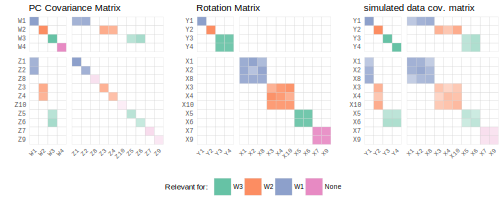
\includegraphics[width=1\linewidth]{Simrel-M_files/figure-latex/cov-plot-print-1} \caption{Simulation of predictor and response variables after orthogonal transformation of principle components by a rotation matrix}\label{fig:cov-plot-print}
\end{figure}

In order to simulate predictor variables \((\mathbf{x})\), we construct
matrix \(\mathbf{R}\) which then is used for orthogonal rotation of
principle components \(\mathbf{z}\). This defines a new basis for the
same space as is spanned by the principle components. In principle,
there are many possible options for a rotation matrix. Among them, the
eigenvector matrix of \(\boldsymbol{\Sigma}_{xx}\) can be a candidate.
However, in this reverse engineering both rotation matrices
\(\mathbf{R}\) and \(\mathbf{Q}\) along with the covariance matrices
\(\boldsymbol{\Sigma}_{xx}\) are unknown. So, we are free to choose any
\(\mathbf{R}\) that satisfied the properties of a real valued rotation
matrix, i.e \(\mathbf{R}^{-1} = \mathbf{R}^t\) so that \(\mathbf{R}\) is
orthonormal and its determinant becomes \(\pm 1\). Here the rotation
matrix \(\mathbf{R}\) should be block diagonal as in
figure\textasciitilde{}\ref{fig:cov-plot-print} (middle) in order to
rotate spaces \(\mathcal{S}_1, \mathcal{S}_2 \ldots\) separately.
Figure\textasciitilde{}\ref{fig:simulated-data} (left) shows the
simulated principle components \(\mathbf{z}\) that we are following in
our example where we can see that the principle component \(z_1\) and
\(z_2\) relevant for \(w_1\) is getting rotated together with an
irrelevant \(z_10\). The resultant predictors
(Figure\textasciitilde{}\ref{fig:simulated-data}, right) \(x_1\),
\(x_2\) and \(x_10\) will also be relevant for \(w_1\). In the figure,
we can see that principle components \(z_8\) and \(z_9\) and
corresponding predictors are not relevant for any of the response.

\begin{figure}
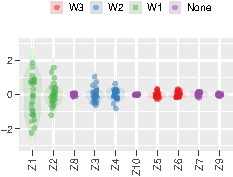
\includegraphics[width=1\linewidth]{Simrel-M_files/figure-latex/simulated-data-1} \caption{Simulated Data before (left) and after (right) rotation}\label{fig:simulated-data}
\end{figure}

Among several methods
\citep{anderson1987generation, heiberger1978algorithm} for generating
random orthogonal matrix, in this paper we are using orthogonal matrix
\(\mathcal{Q}\) obtained from QR-decomposition of a matrix filled with
standard normal variate. The rotation here can be a) restricted and b)
unrestricted. The later one rotates all principle components
\(\mathbf{z}\) together and makes all predictor variables somewhat
relevant for all response variables. However, the former one performs a
block-wise rotation so that it rotates certain selected principle
components together. This gives control for specifying certain
predictors as relevant for selected response, which was discussed in our
example above. This also lets us to simulate irrelevant predictors such
as \(x_7\) and \(x_8\) which can be detected during variables selection
procedure.

\section*{References}\label{references}
\addcontentsline{toc}{section}{References}


\renewcommand\refname{References}
\bibliography{packages.bib,ref-db.bib}



\end{document}
